\documentclass[twoside]{book}

% Packages required by doxygen
\usepackage{fixltx2e}
\usepackage{calc}
\usepackage{doxygen}
\usepackage[export]{adjustbox} % also loads graphicx
\usepackage{graphicx}
\usepackage[utf8]{inputenc}
\usepackage{makeidx}
\usepackage{multicol}
\usepackage{multirow}
\PassOptionsToPackage{warn}{textcomp}
\usepackage{textcomp}
\usepackage[nointegrals]{wasysym}
\usepackage[table]{xcolor}

% Font selection
\usepackage[T1]{fontenc}
\usepackage[scaled=.90]{helvet}
\usepackage{courier}
\usepackage{amssymb}
\usepackage{sectsty}
\renewcommand{\familydefault}{\sfdefault}
\allsectionsfont{%
  \fontseries{bc}\selectfont%
  \color{darkgray}%
}
\renewcommand{\DoxyLabelFont}{%
  \fontseries{bc}\selectfont%
  \color{darkgray}%
}
\newcommand{\+}{\discretionary{\mbox{\scriptsize$\hookleftarrow$}}{}{}}

% Page & text layout
\usepackage{geometry}
\geometry{%
  a4paper,%
  top=2.5cm,%
  bottom=2.5cm,%
  left=2.5cm,%
  right=2.5cm%
}
\tolerance=750
\hfuzz=15pt
\hbadness=750
\setlength{\emergencystretch}{15pt}
\setlength{\parindent}{0cm}
\setlength{\parskip}{3ex plus 2ex minus 2ex}
\makeatletter
\renewcommand{\paragraph}{%
  \@startsection{paragraph}{4}{0ex}{-1.0ex}{1.0ex}{%
    \normalfont\normalsize\bfseries\SS@parafont%
  }%
}
\renewcommand{\subparagraph}{%
  \@startsection{subparagraph}{5}{0ex}{-1.0ex}{1.0ex}{%
    \normalfont\normalsize\bfseries\SS@subparafont%
  }%
}
\makeatother

% Headers & footers
\usepackage{fancyhdr}
\pagestyle{fancyplain}
\fancyhead[LE]{\fancyplain{}{\bfseries\thepage}}
\fancyhead[CE]{\fancyplain{}{}}
\fancyhead[RE]{\fancyplain{}{\bfseries\leftmark}}
\fancyhead[LO]{\fancyplain{}{\bfseries\rightmark}}
\fancyhead[CO]{\fancyplain{}{}}
\fancyhead[RO]{\fancyplain{}{\bfseries\thepage}}
\fancyfoot[LE]{\fancyplain{}{}}
\fancyfoot[CE]{\fancyplain{}{}}
\fancyfoot[RE]{\fancyplain{}{\bfseries\scriptsize Generated by Doxygen }}
\fancyfoot[LO]{\fancyplain{}{\bfseries\scriptsize Generated by Doxygen }}
\fancyfoot[CO]{\fancyplain{}{}}
\fancyfoot[RO]{\fancyplain{}{}}
\renewcommand{\footrulewidth}{0.4pt}
\renewcommand{\chaptermark}[1]{%
  \markboth{#1}{}%
}
\renewcommand{\sectionmark}[1]{%
  \markright{\thesection\ #1}%
}

% Indices & bibliography
\usepackage{natbib}
\usepackage[titles]{tocloft}
\setcounter{tocdepth}{3}
\setcounter{secnumdepth}{5}
\makeindex

% Hyperlinks (required, but should be loaded last)
\usepackage{ifpdf}
\ifpdf
  \usepackage[pdftex,pagebackref=true]{hyperref}
\else
  \usepackage[ps2pdf,pagebackref=true]{hyperref}
\fi
\hypersetup{%
  colorlinks=true,%
  linkcolor=blue,%
  citecolor=blue,%
  unicode%
}

% Custom commands
\newcommand{\clearemptydoublepage}{%
  \newpage{\pagestyle{empty}\cleardoublepage}%
}

\usepackage{caption}
\captionsetup{labelsep=space,justification=centering,font={bf},singlelinecheck=off,skip=4pt,position=top}

%===== C O N T E N T S =====

\begin{document}

% Titlepage & ToC
\hypersetup{pageanchor=false,
             bookmarksnumbered=true,
             pdfencoding=unicode
            }
\pagenumbering{alph}
\begin{titlepage}
\vspace*{7cm}
\begin{center}%
{\Large My Project }\\
\vspace*{1cm}
{\large Generated by Doxygen 1.8.13}\\
\end{center}
\end{titlepage}
\clearemptydoublepage
\pagenumbering{roman}
\tableofcontents
\clearemptydoublepage
\pagenumbering{arabic}
\hypersetup{pageanchor=true}

%--- Begin generated contents ---
\chapter{tsap}
\label{md__u_qingcanw_Programs_tsap_README}
\Hypertarget{md__u_qingcanw_Programs_tsap_README}




Time series analysis in python A\+PC 524, Fall 2016, Final project Project members\+: Wenyan Gong, Zongxi Li, Cong Ma, Qingcan Wang, Zhuoran Yang, Hao Zhang





In this project, we will develop a python module that provides tools for time series analysis. We provide python class in src/ folder. 
\chapter{Hierarchical Index}
\section{Class Hierarchy}
This inheritance list is sorted roughly, but not completely, alphabetically\+:\begin{DoxyCompactList}
\item object\begin{DoxyCompactList}
\item \contentsline{section}{src.\+basemodel.\+base}{\pageref{classsrc_1_1basemodel_1_1base}}{}
\begin{DoxyCompactList}
\item \contentsline{section}{src.\+model.\+AR}{\pageref{classsrc_1_1model_1_1AR}}{}
\item \contentsline{section}{src.\+model.\+MA}{\pageref{classsrc_1_1model_1_1MA}}{}
\end{DoxyCompactList}
\item \contentsline{section}{src.\+cluster.\+Cluster}{\pageref{classsrc_1_1cluster_1_1Cluster}}{}
\item \contentsline{section}{src.\+option\+Pricing.\+Option\+Pricing}{\pageref{classsrc_1_1optionPricing_1_1OptionPricing}}{}
\item \contentsline{section}{src.\+reduction.\+Reduction}{\pageref{classsrc_1_1reduction_1_1Reduction}}{}
\item \contentsline{section}{src.\+solver.\+Solver}{\pageref{classsrc_1_1solver_1_1Solver}}{}
\end{DoxyCompactList}
\item Test\+Case\begin{DoxyCompactList}
\item \contentsline{section}{test.\+testdataprocessor.\+Test\+Data\+Processor}{\pageref{classtest_1_1testdataprocessor_1_1TestDataProcessor}}{}
\item \contentsline{section}{test.\+testmodel.\+Test\+Model}{\pageref{classtest_1_1testmodel_1_1TestModel}}{}
\item \contentsline{section}{test.\+testtrading.\+Test\+Trading}{\pageref{classtest_1_1testtrading_1_1TestTrading}}{}
\end{DoxyCompactList}
\end{DoxyCompactList}

\chapter{Class Index}
\section{Class List}
Here are the classes, structs, unions and interfaces with brief descriptions\+:\begin{DoxyCompactList}
\item\contentsline{section}{\hyperlink{classsrc_1_1model_1_1AR}{src.\+model.\+AR} }{\pageref{classsrc_1_1model_1_1AR}}{}
\item\contentsline{section}{\hyperlink{classsrc_1_1basemodel_1_1base}{src.\+basemodel.\+base} }{\pageref{classsrc_1_1basemodel_1_1base}}{}
\item\contentsline{section}{\hyperlink{classsrc_1_1cluster_1_1Cluster}{src.\+cluster.\+Cluster} }{\pageref{classsrc_1_1cluster_1_1Cluster}}{}
\item\contentsline{section}{\hyperlink{classsrc_1_1model_1_1MA}{src.\+model.\+MA} }{\pageref{classsrc_1_1model_1_1MA}}{}
\item\contentsline{section}{\hyperlink{classsrc_1_1optionPricing_1_1OptionPricing}{src.\+option\+Pricing.\+Option\+Pricing} }{\pageref{classsrc_1_1optionPricing_1_1OptionPricing}}{}
\item\contentsline{section}{\hyperlink{classsrc_1_1reduction_1_1Reduction}{src.\+reduction.\+Reduction} }{\pageref{classsrc_1_1reduction_1_1Reduction}}{}
\item\contentsline{section}{\hyperlink{classsrc_1_1solver_1_1Solver}{src.\+solver.\+Solver} }{\pageref{classsrc_1_1solver_1_1Solver}}{}
\item\contentsline{section}{\hyperlink{classtest_1_1testdataprocessor_1_1TestDataProcessor}{test.\+testdataprocessor.\+Test\+Data\+Processor} }{\pageref{classtest_1_1testdataprocessor_1_1TestDataProcessor}}{}
\item\contentsline{section}{\hyperlink{classtest_1_1testmodel_1_1TestModel}{test.\+testmodel.\+Test\+Model} }{\pageref{classtest_1_1testmodel_1_1TestModel}}{}
\item\contentsline{section}{\hyperlink{classtest_1_1testtrading_1_1TestTrading}{test.\+testtrading.\+Test\+Trading} }{\pageref{classtest_1_1testtrading_1_1TestTrading}}{}
\end{DoxyCompactList}

\chapter{Class Documentation}
\hypertarget{classsrc_1_1model_1_1AR}{}\section{src.\+model.\+AR Class Reference}
\label{classsrc_1_1model_1_1AR}\index{src.\+model.\+AR@{src.\+model.\+AR}}
Inheritance diagram for src.\+model.\+AR\+:\begin{figure}[H]
\begin{center}
\leavevmode
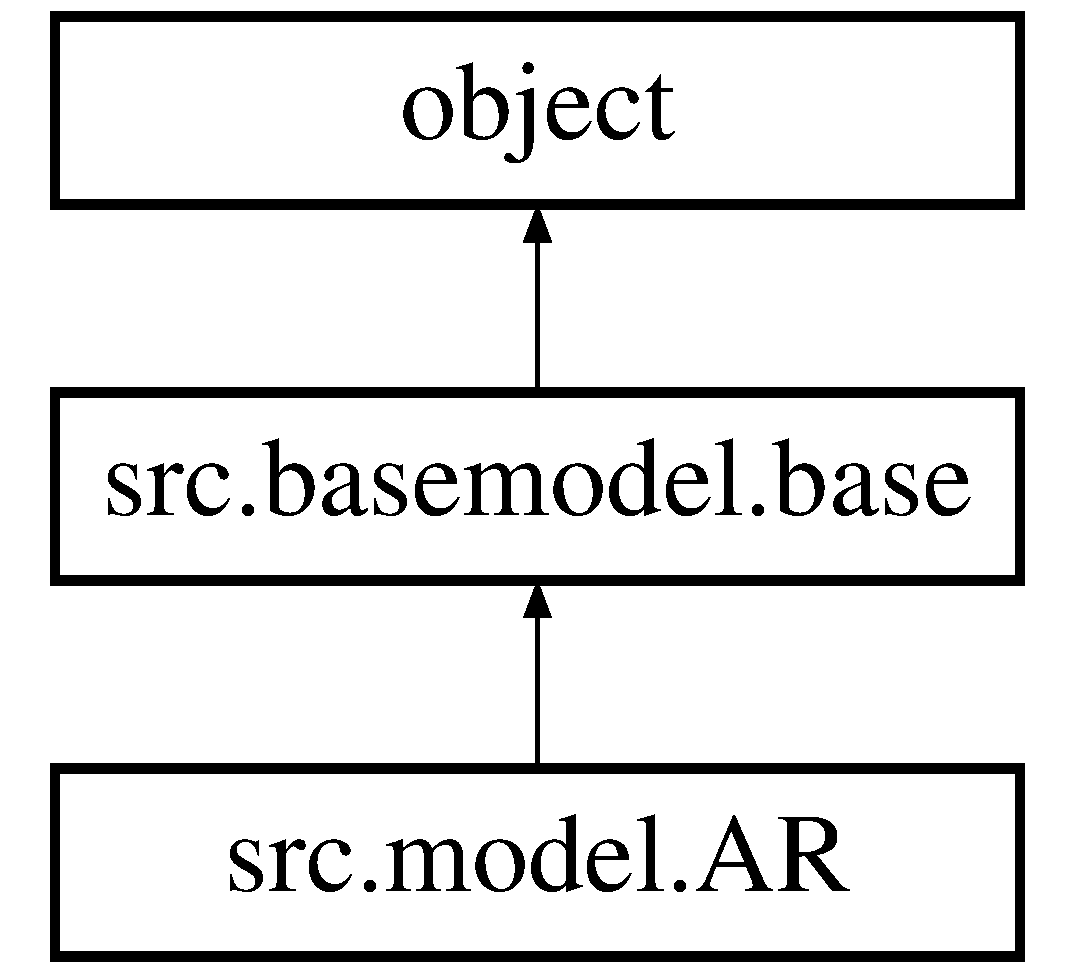
\includegraphics[height=3.000000cm]{classsrc_1_1model_1_1AR}
\end{center}
\end{figure}
\subsection*{Public Member Functions}
\begin{DoxyCompactItemize}
\item 
def \hyperlink{classsrc_1_1model_1_1AR_a943f799da7cba763b29778ba12481c64}{\+\_\+\+\_\+init\+\_\+\+\_\+} (self, lag, phi, sigma, intercept)
\item 
def \hyperlink{classsrc_1_1model_1_1AR_ae6095b1c295bdbd6dddd0b1fa87948ef}{loss} (self, X, lag=None, phi=None, sigma=None, intercept=None)
\item 
def \hyperlink{classsrc_1_1model_1_1AR_a2a2f41f1e5cfb10f0c5680ea689e1994}{predict} (self, X, nstep, lag=None, phi=None, sigma=None, intercept=None)
\end{DoxyCompactItemize}
\subsection*{Public Attributes}
\begin{DoxyCompactItemize}
\item 
\mbox{\Hypertarget{classsrc_1_1model_1_1AR_a4ba754929f5fa9b24a5b6653d7b62411}\label{classsrc_1_1model_1_1AR_a4ba754929f5fa9b24a5b6653d7b62411}} 
{\bfseries params}
\end{DoxyCompactItemize}


\subsection{Detailed Description}
\begin{DoxyVerb}class AR implements the AR model which has __init__ , loss and predict as functions\end{DoxyVerb}
 

\subsection{Constructor \& Destructor Documentation}
\mbox{\Hypertarget{classsrc_1_1model_1_1AR_a943f799da7cba763b29778ba12481c64}\label{classsrc_1_1model_1_1AR_a943f799da7cba763b29778ba12481c64}} 
\index{src\+::model\+::\+AR@{src\+::model\+::\+AR}!\+\_\+\+\_\+init\+\_\+\+\_\+@{\+\_\+\+\_\+init\+\_\+\+\_\+}}
\index{\+\_\+\+\_\+init\+\_\+\+\_\+@{\+\_\+\+\_\+init\+\_\+\+\_\+}!src\+::model\+::\+AR@{src\+::model\+::\+AR}}
\subsubsection{\texorpdfstring{\+\_\+\+\_\+init\+\_\+\+\_\+()}{\_\_init\_\_()}}
{\footnotesize\ttfamily def src.\+model.\+A\+R.\+\_\+\+\_\+init\+\_\+\+\_\+ (\begin{DoxyParamCaption}\item[{}]{self,  }\item[{}]{lag,  }\item[{}]{phi,  }\item[{}]{sigma,  }\item[{}]{intercept }\end{DoxyParamCaption})}

\begin{DoxyVerb}__init__: initialize the model with lag phi sigma and intercept
   Input: 
 lag: the number of lag in AR model, dimension 1
 phi: the coefficients for each lag, dimension lag, column vector
 sigma: the standard deviation of the error term, dimension 1
 intercept: the constant component in the AR model, dimension 1
   Output:
 _lag: the number of lag in the AR model
 params: hash table of phi, sigma and intercept\end{DoxyVerb}
 

\subsection{Member Function Documentation}
\mbox{\Hypertarget{classsrc_1_1model_1_1AR_ae6095b1c295bdbd6dddd0b1fa87948ef}\label{classsrc_1_1model_1_1AR_ae6095b1c295bdbd6dddd0b1fa87948ef}} 
\index{src\+::model\+::\+AR@{src\+::model\+::\+AR}!loss@{loss}}
\index{loss@{loss}!src\+::model\+::\+AR@{src\+::model\+::\+AR}}
\subsubsection{\texorpdfstring{loss()}{loss()}}
{\footnotesize\ttfamily def src.\+model.\+A\+R.\+loss (\begin{DoxyParamCaption}\item[{}]{self,  }\item[{}]{X,  }\item[{}]{lag = {\ttfamily None},  }\item[{}]{phi = {\ttfamily None},  }\item[{}]{sigma = {\ttfamily None},  }\item[{}]{intercept = {\ttfamily None} }\end{DoxyParamCaption})}

\begin{DoxyVerb}loss: return the loglikelihood and its gradient with respect to phi, sigma and intercept
   Input: 
 X: the input time series, each row is about one stock. For one stock, X is a row vector. Note phi is a column vector
   Output:
  loglikelihood: the loglikelihood that calculated from the input time series
  grads: hash table that records the gradient of phi sigma and intercept\end{DoxyVerb}
\begin{DoxyVerb}the number of samples, usually it's about how many stocks we have \end{DoxyVerb}
 \mbox{\Hypertarget{classsrc_1_1model_1_1AR_a2a2f41f1e5cfb10f0c5680ea689e1994}\label{classsrc_1_1model_1_1AR_a2a2f41f1e5cfb10f0c5680ea689e1994}} 
\index{src\+::model\+::\+AR@{src\+::model\+::\+AR}!predict@{predict}}
\index{predict@{predict}!src\+::model\+::\+AR@{src\+::model\+::\+AR}}
\subsubsection{\texorpdfstring{predict()}{predict()}}
{\footnotesize\ttfamily def src.\+model.\+A\+R.\+predict (\begin{DoxyParamCaption}\item[{}]{self,  }\item[{}]{X,  }\item[{}]{nstep,  }\item[{}]{lag = {\ttfamily None},  }\item[{}]{phi = {\ttfamily None},  }\item[{}]{sigma = {\ttfamily None},  }\item[{}]{intercept = {\ttfamily None} }\end{DoxyParamCaption})}

\begin{DoxyVerb}predict: return the predicted series based on the samples given
   Input: 
 X: the input time series, each row is about one stock. For one stock, X is a row vector. Note phi is a column vector
 nstep: the number of steps to predict
   Output:
  pred_state: the predicted series based on AR model, which is a row vector\end{DoxyVerb}
\begin{DoxyVerb}parameters\end{DoxyVerb}
 

The documentation for this class was generated from the following file\+:\begin{DoxyCompactItemize}
\item 
/u/qingcanw/\+Programs/tsap/src/model.\+py\end{DoxyCompactItemize}

\hypertarget{classsrc_1_1basemodel_1_1base}{}\section{src.\+basemodel.\+base Class Reference}
\label{classsrc_1_1basemodel_1_1base}\index{src.\+basemodel.\+base@{src.\+basemodel.\+base}}
Inheritance diagram for src.\+basemodel.\+base\+:\begin{figure}[H]
\begin{center}
\leavevmode
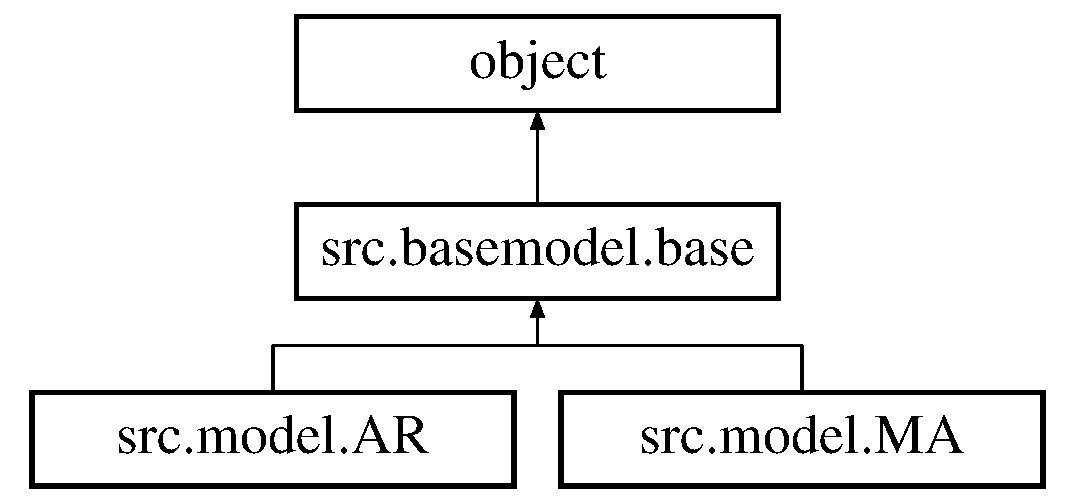
\includegraphics[height=3.000000cm]{classsrc_1_1basemodel_1_1base}
\end{center}
\end{figure}
\subsection*{Public Member Functions}
\begin{DoxyCompactItemize}
\item 
\mbox{\Hypertarget{classsrc_1_1basemodel_1_1base_abecfbc88023bb6a31cac29f7d3e94bba}\label{classsrc_1_1basemodel_1_1base_abecfbc88023bb6a31cac29f7d3e94bba}} 
def {\bfseries \+\_\+\+\_\+init\+\_\+\+\_\+} (self)
\item 
\mbox{\Hypertarget{classsrc_1_1basemodel_1_1base_aeffdc26cfd3f8132b12841e8fb3f9ffe}\label{classsrc_1_1basemodel_1_1base_aeffdc26cfd3f8132b12841e8fb3f9ffe}} 
def {\bfseries loss} (self, X)
\item 
\mbox{\Hypertarget{classsrc_1_1basemodel_1_1base_a06ef519662cbfefdd0c2760ba6b4d496}\label{classsrc_1_1basemodel_1_1base_a06ef519662cbfefdd0c2760ba6b4d496}} 
def {\bfseries predict} (self, X, nstep)
\end{DoxyCompactItemize}


The documentation for this class was generated from the following file\+:\begin{DoxyCompactItemize}
\item 
/u/qingcanw/\+Programs/tsap/src/basemodel.\+py\end{DoxyCompactItemize}

\hypertarget{classsrc_1_1cluster_1_1Cluster}{}\section{src.\+cluster.\+Cluster Class Reference}
\label{classsrc_1_1cluster_1_1Cluster}\index{src.\+cluster.\+Cluster@{src.\+cluster.\+Cluster}}
Inheritance diagram for src.\+cluster.\+Cluster\+:\begin{figure}[H]
\begin{center}
\leavevmode
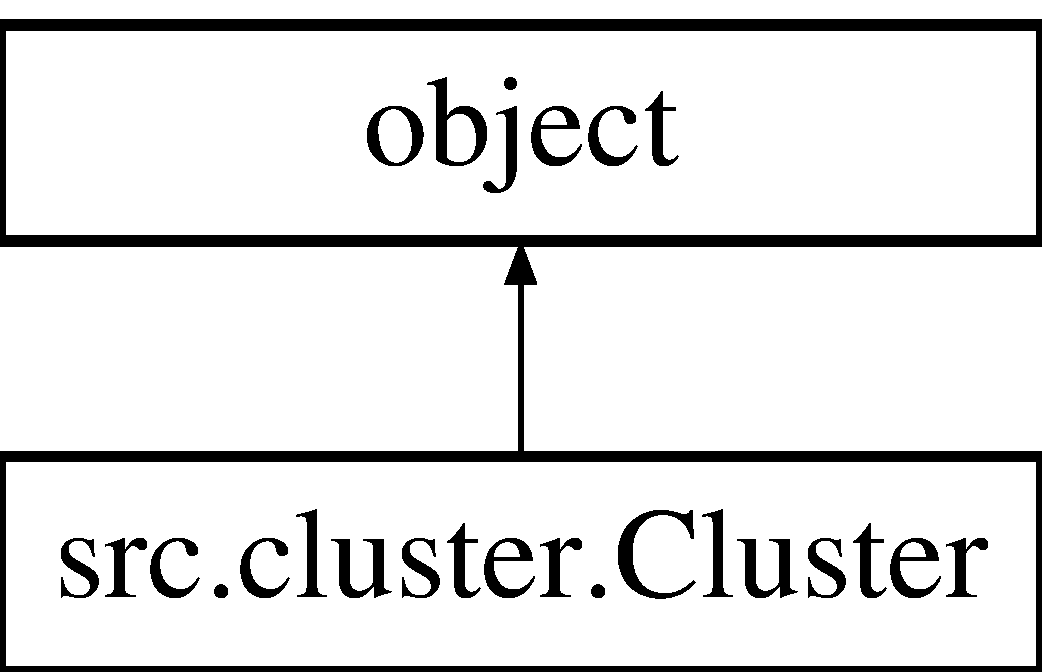
\includegraphics[height=2.000000cm]{classsrc_1_1cluster_1_1Cluster}
\end{center}
\end{figure}
\subsection*{Public Member Functions}
\begin{DoxyCompactItemize}
\item 
def \hyperlink{classsrc_1_1cluster_1_1Cluster_aecb660a329d008897008ccb17a49f349}{\+\_\+\+\_\+init\+\_\+\+\_\+} (self, X)
\item 
def \hyperlink{classsrc_1_1cluster_1_1Cluster_a8cb50b6db992f7a5c686c0d00fb2343a}{assign\+\_\+label} (self, Centers)
\item 
def \hyperlink{classsrc_1_1cluster_1_1Cluster_afd29b7a67da864dbc7b8352e8ed0cdab}{k\+Means} (self, n\+Clusters, max\+Iter=300)
\end{DoxyCompactItemize}


\subsection{Constructor \& Destructor Documentation}
\mbox{\Hypertarget{classsrc_1_1cluster_1_1Cluster_aecb660a329d008897008ccb17a49f349}\label{classsrc_1_1cluster_1_1Cluster_aecb660a329d008897008ccb17a49f349}} 
\index{src\+::cluster\+::\+Cluster@{src\+::cluster\+::\+Cluster}!\+\_\+\+\_\+init\+\_\+\+\_\+@{\+\_\+\+\_\+init\+\_\+\+\_\+}}
\index{\+\_\+\+\_\+init\+\_\+\+\_\+@{\+\_\+\+\_\+init\+\_\+\+\_\+}!src\+::cluster\+::\+Cluster@{src\+::cluster\+::\+Cluster}}
\subsubsection{\texorpdfstring{\+\_\+\+\_\+init\+\_\+\+\_\+()}{\_\_init\_\_()}}
{\footnotesize\ttfamily def src.\+cluster.\+Cluster.\+\_\+\+\_\+init\+\_\+\+\_\+ (\begin{DoxyParamCaption}\item[{}]{self,  }\item[{}]{X }\end{DoxyParamCaption})}

\begin{DoxyVerb}Return a new object to cluster data based on selected clutering
algorithm.
Example usage: clusterObj = Clustering(X)
X:     numpy array, shape (n_samples, n_features)\end{DoxyVerb}
 

\subsection{Member Function Documentation}
\mbox{\Hypertarget{classsrc_1_1cluster_1_1Cluster_a8cb50b6db992f7a5c686c0d00fb2343a}\label{classsrc_1_1cluster_1_1Cluster_a8cb50b6db992f7a5c686c0d00fb2343a}} 
\index{src\+::cluster\+::\+Cluster@{src\+::cluster\+::\+Cluster}!assign\+\_\+label@{assign\+\_\+label}}
\index{assign\+\_\+label@{assign\+\_\+label}!src\+::cluster\+::\+Cluster@{src\+::cluster\+::\+Cluster}}
\subsubsection{\texorpdfstring{assign\+\_\+label()}{assign\_label()}}
{\footnotesize\ttfamily def src.\+cluster.\+Cluster.\+assign\+\_\+label (\begin{DoxyParamCaption}\item[{}]{self,  }\item[{}]{Centers }\end{DoxyParamCaption})}

\begin{DoxyVerb}Assign labels to the data points
    Input:
self
Centers:  numpy array, shape (n_clusters, n_features) the centers of each cluster
    Output:
clusters: the index of data points in each class
labels: the label of each class\end{DoxyVerb}
 \mbox{\Hypertarget{classsrc_1_1cluster_1_1Cluster_afd29b7a67da864dbc7b8352e8ed0cdab}\label{classsrc_1_1cluster_1_1Cluster_afd29b7a67da864dbc7b8352e8ed0cdab}} 
\index{src\+::cluster\+::\+Cluster@{src\+::cluster\+::\+Cluster}!k\+Means@{k\+Means}}
\index{k\+Means@{k\+Means}!src\+::cluster\+::\+Cluster@{src\+::cluster\+::\+Cluster}}
\subsubsection{\texorpdfstring{k\+Means()}{kMeans()}}
{\footnotesize\ttfamily def src.\+cluster.\+Cluster.\+k\+Means (\begin{DoxyParamCaption}\item[{}]{self,  }\item[{}]{n\+Clusters,  }\item[{}]{max\+Iter = {\ttfamily 300} }\end{DoxyParamCaption})}

\begin{DoxyVerb}K-means clustering algorithm.

Function usage: kMeans(nClusters, maxIter, nInit)

Inputs:
nClusters : int
    The number of clusters to form as well as the number of
    centroids to generate.
maxIter : int, optional, default 300
    Maximum number of iterations of the k-means algorithm to run.

Returns:
centroid :  float ndarray with shape (k, n_features)
    Centroids found at the last iteration of k-means.
label : integer ndarray with shape (n_samples,)
    label[i] is the code or index of the centroid the i’th
    observation is closest to.
inertia : float
    The final value of the inertia criterion (sum of squared
    distances to the closest centroid for all observations
    in the training set).\end{DoxyVerb}
 

The documentation for this class was generated from the following file\+:\begin{DoxyCompactItemize}
\item 
/u/qingcanw/\+Programs/tsap/src/cluster.\+py\end{DoxyCompactItemize}

\hypertarget{classsrc_1_1model_1_1MA}{}\section{src.\+model.\+MA Class Reference}
\label{classsrc_1_1model_1_1MA}\index{src.\+model.\+MA@{src.\+model.\+MA}}
Inheritance diagram for src.\+model.\+MA\+:\begin{figure}[H]
\begin{center}
\leavevmode
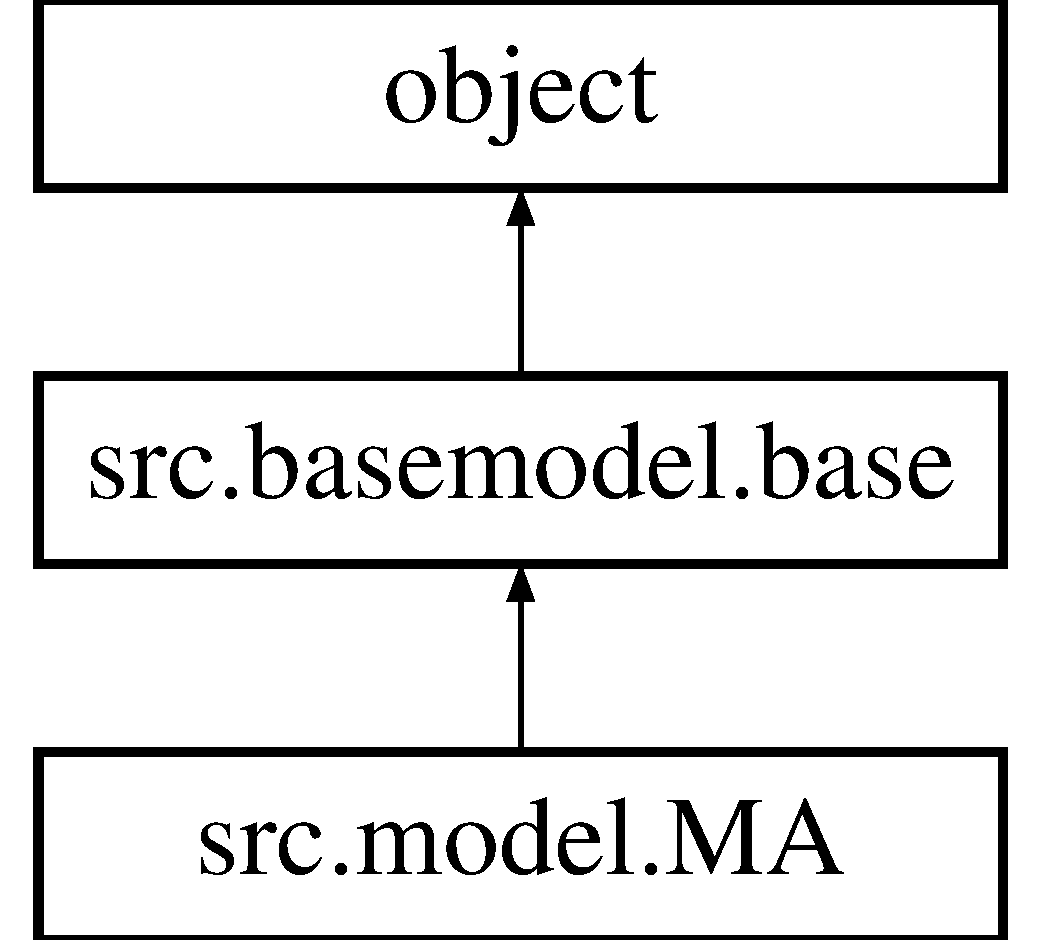
\includegraphics[height=3.000000cm]{classsrc_1_1model_1_1MA}
\end{center}
\end{figure}
\subsection*{Public Member Functions}
\begin{DoxyCompactItemize}
\item 
def \hyperlink{classsrc_1_1model_1_1MA_a6a4df2f2b129069362819f597a1fc672}{\+\_\+\+\_\+init\+\_\+\+\_\+} (self, lag, phi, sigma, intercept)
\item 
\mbox{\Hypertarget{classsrc_1_1model_1_1MA_a928e833a902d658a3f6b8ffe1cea02ee}\label{classsrc_1_1model_1_1MA_a928e833a902d658a3f6b8ffe1cea02ee}} 
def {\bfseries loss} (self, X, lag=None, phi=None, sigma=None, intercept=None)
\item 
def \hyperlink{classsrc_1_1model_1_1MA_ac4f9c0e95e6a26447797a9e82144311c}{get\+\_\+loglikelihood} (self, X, lag=None, phi=None, sigma=None, intercept=None)
\item 
def \hyperlink{classsrc_1_1model_1_1MA_af0d3f5582d13a5b653b7b3ca5a5c2c68}{predict} (self, X, nstep)
\end{DoxyCompactItemize}
\subsection*{Public Attributes}
\begin{DoxyCompactItemize}
\item 
\mbox{\Hypertarget{classsrc_1_1model_1_1MA_ad68f02ab2e17d6c9e2c7ab74403d87ac}\label{classsrc_1_1model_1_1MA_ad68f02ab2e17d6c9e2c7ab74403d87ac}} 
{\bfseries params}
\end{DoxyCompactItemize}


\subsection{Constructor \& Destructor Documentation}
\mbox{\Hypertarget{classsrc_1_1model_1_1MA_a6a4df2f2b129069362819f597a1fc672}\label{classsrc_1_1model_1_1MA_a6a4df2f2b129069362819f597a1fc672}} 
\index{src\+::model\+::\+MA@{src\+::model\+::\+MA}!\+\_\+\+\_\+init\+\_\+\+\_\+@{\+\_\+\+\_\+init\+\_\+\+\_\+}}
\index{\+\_\+\+\_\+init\+\_\+\+\_\+@{\+\_\+\+\_\+init\+\_\+\+\_\+}!src\+::model\+::\+MA@{src\+::model\+::\+MA}}
\subsubsection{\texorpdfstring{\+\_\+\+\_\+init\+\_\+\+\_\+()}{\_\_init\_\_()}}
{\footnotesize\ttfamily def src.\+model.\+M\+A.\+\_\+\+\_\+init\+\_\+\+\_\+ (\begin{DoxyParamCaption}\item[{}]{self,  }\item[{}]{lag,  }\item[{}]{phi,  }\item[{}]{sigma,  }\item[{}]{intercept }\end{DoxyParamCaption})}

\begin{DoxyVerb}lag, phi, sigma, intercept is the parameter of AR\end{DoxyVerb}
 

\subsection{Member Function Documentation}
\mbox{\Hypertarget{classsrc_1_1model_1_1MA_ac4f9c0e95e6a26447797a9e82144311c}\label{classsrc_1_1model_1_1MA_ac4f9c0e95e6a26447797a9e82144311c}} 
\index{src\+::model\+::\+MA@{src\+::model\+::\+MA}!get\+\_\+loglikelihood@{get\+\_\+loglikelihood}}
\index{get\+\_\+loglikelihood@{get\+\_\+loglikelihood}!src\+::model\+::\+MA@{src\+::model\+::\+MA}}
\subsubsection{\texorpdfstring{get\+\_\+loglikelihood()}{get\_loglikelihood()}}
{\footnotesize\ttfamily def src.\+model.\+M\+A.\+get\+\_\+loglikelihood (\begin{DoxyParamCaption}\item[{}]{self,  }\item[{}]{X,  }\item[{}]{lag = {\ttfamily None},  }\item[{}]{phi = {\ttfamily None},  }\item[{}]{sigma = {\ttfamily None},  }\item[{}]{intercept = {\ttfamily None} }\end{DoxyParamCaption})}

\begin{DoxyVerb}X is dataset, right now X is a row vector\end{DoxyVerb}
\begin{DoxyVerb}phi is a column vector, and we need to make it into matrix form\end{DoxyVerb}
 \mbox{\Hypertarget{classsrc_1_1model_1_1MA_af0d3f5582d13a5b653b7b3ca5a5c2c68}\label{classsrc_1_1model_1_1MA_af0d3f5582d13a5b653b7b3ca5a5c2c68}} 
\index{src\+::model\+::\+MA@{src\+::model\+::\+MA}!predict@{predict}}
\index{predict@{predict}!src\+::model\+::\+MA@{src\+::model\+::\+MA}}
\subsubsection{\texorpdfstring{predict()}{predict()}}
{\footnotesize\ttfamily def src.\+model.\+M\+A.\+predict (\begin{DoxyParamCaption}\item[{}]{self,  }\item[{}]{X,  }\item[{}]{nstep }\end{DoxyParamCaption})}

\begin{DoxyVerb}X is a row vector\end{DoxyVerb}
 

The documentation for this class was generated from the following file\+:\begin{DoxyCompactItemize}
\item 
/u/qingcanw/\+Programs/tsap/src/model.\+py\end{DoxyCompactItemize}

\hypertarget{classsrc_1_1optionPricing_1_1OptionPricing}{}\section{src.\+option\+Pricing.\+Option\+Pricing Class Reference}
\label{classsrc_1_1optionPricing_1_1OptionPricing}\index{src.\+option\+Pricing.\+Option\+Pricing@{src.\+option\+Pricing.\+Option\+Pricing}}
Inheritance diagram for src.\+option\+Pricing.\+Option\+Pricing\+:\begin{figure}[H]
\begin{center}
\leavevmode
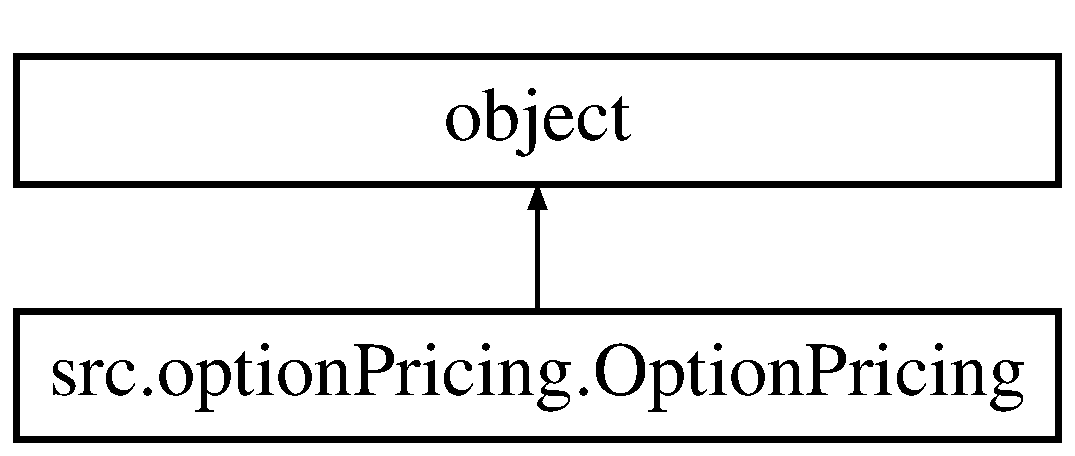
\includegraphics[height=2.000000cm]{classsrc_1_1optionPricing_1_1OptionPricing}
\end{center}
\end{figure}
\subsection*{Public Member Functions}
\begin{DoxyCompactItemize}
\item 
\mbox{\Hypertarget{classsrc_1_1optionPricing_1_1OptionPricing_a4642cf5de43033ea6af43adb2bd79b49}\label{classsrc_1_1optionPricing_1_1OptionPricing_a4642cf5de43033ea6af43adb2bd79b49}} 
def {\bfseries \+\_\+\+\_\+init\+\_\+\+\_\+} (self, sigma=0.\+1, r=0.\+01, T=1, K=1, Smax=None, Vmax=None)
\item 
def \hyperlink{classsrc_1_1optionPricing_1_1OptionPricing_a5ee60e0ef4ec623ffca945b42d21c567}{Black\+Scholes\+Eqn} (self, dS, dt)
\item 
def \hyperlink{classsrc_1_1optionPricing_1_1OptionPricing_affc466184874e04ddc6deae50c50e8eb}{option\+Price} (self, V, S, t)
\end{DoxyCompactItemize}


\subsection{Detailed Description}
\begin{DoxyVerb}Callable option pricing object.
Example usage:
optionPriceobj = optionPricing(sigma,r,T,K), declare a class object
V = optionPriceobj.BlackScholesEqn(dS,dt), compute V array in shape [nS,nt]
Vst = optionPriceobj.optionPrice(V,S,t), compute V(S,t) given V array
\end{DoxyVerb}
 

\subsection{Member Function Documentation}
\mbox{\Hypertarget{classsrc_1_1optionPricing_1_1OptionPricing_a5ee60e0ef4ec623ffca945b42d21c567}\label{classsrc_1_1optionPricing_1_1OptionPricing_a5ee60e0ef4ec623ffca945b42d21c567}} 
\index{src\+::option\+Pricing\+::\+Option\+Pricing@{src\+::option\+Pricing\+::\+Option\+Pricing}!Black\+Scholes\+Eqn@{Black\+Scholes\+Eqn}}
\index{Black\+Scholes\+Eqn@{Black\+Scholes\+Eqn}!src\+::option\+Pricing\+::\+Option\+Pricing@{src\+::option\+Pricing\+::\+Option\+Pricing}}
\subsubsection{\texorpdfstring{Black\+Scholes\+Eqn()}{BlackScholesEqn()}}
{\footnotesize\ttfamily def src.\+option\+Pricing.\+Option\+Pricing.\+Black\+Scholes\+Eqn (\begin{DoxyParamCaption}\item[{}]{self,  }\item[{}]{dS,  }\item[{}]{dt }\end{DoxyParamCaption})}

\begin{DoxyVerb}V(S, t) satisfies Black-Scholes equation
dVdt + (1/2)*sigma^2*S^2*d2VdS2 + r*S*dVdS - r*V = 0

Inputs:
dS: float, size of grids in S dimension
dt: float, size of grids in t dimension

Returns:
V: array, shape [nS, nt]
\end{DoxyVerb}
 \mbox{\Hypertarget{classsrc_1_1optionPricing_1_1OptionPricing_affc466184874e04ddc6deae50c50e8eb}\label{classsrc_1_1optionPricing_1_1OptionPricing_affc466184874e04ddc6deae50c50e8eb}} 
\index{src\+::option\+Pricing\+::\+Option\+Pricing@{src\+::option\+Pricing\+::\+Option\+Pricing}!option\+Price@{option\+Price}}
\index{option\+Price@{option\+Price}!src\+::option\+Pricing\+::\+Option\+Pricing@{src\+::option\+Pricing\+::\+Option\+Pricing}}
\subsubsection{\texorpdfstring{option\+Price()}{optionPrice()}}
{\footnotesize\ttfamily def src.\+option\+Pricing.\+Option\+Pricing.\+option\+Price (\begin{DoxyParamCaption}\item[{}]{self,  }\item[{}]{V,  }\item[{}]{S,  }\item[{}]{t }\end{DoxyParamCaption})}

\begin{DoxyVerb}Given discrete V arrary in shape [nS, nt], compute V at V(S,t) by 
simple interpolation
Inputs:
V: array in shape [nS, nt]
S: stock price
t: time
Returns:
VSt: option price V(S,t)
\end{DoxyVerb}
 

The documentation for this class was generated from the following file\+:\begin{DoxyCompactItemize}
\item 
/u/qingcanw/\+Programs/tsap/src/option\+Pricing.\+py\end{DoxyCompactItemize}

\hypertarget{classsrc_1_1reduction_1_1Reduction}{}\section{src.\+reduction.\+Reduction Class Reference}
\label{classsrc_1_1reduction_1_1Reduction}\index{src.\+reduction.\+Reduction@{src.\+reduction.\+Reduction}}
Inheritance diagram for src.\+reduction.\+Reduction\+:\begin{figure}[H]
\begin{center}
\leavevmode
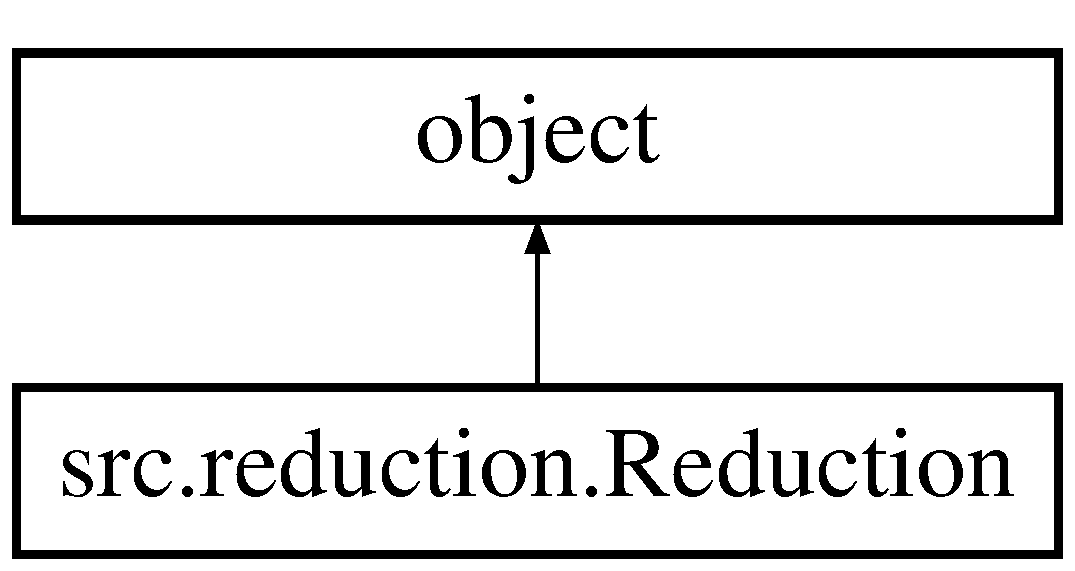
\includegraphics[height=2.000000cm]{classsrc_1_1reduction_1_1Reduction}
\end{center}
\end{figure}
\subsection*{Public Member Functions}
\begin{DoxyCompactItemize}
\item 
\mbox{\Hypertarget{classsrc_1_1reduction_1_1Reduction_ab7ff5ded32de74d8ac34302ecc9b0b71}\label{classsrc_1_1reduction_1_1Reduction_ab7ff5ded32de74d8ac34302ecc9b0b71}} 
def {\bfseries \+\_\+\+\_\+init\+\_\+\+\_\+} (self, X)
\item 
def \hyperlink{classsrc_1_1reduction_1_1Reduction_ac81be4ff2c47e70a5f0af081af6faff6}{P\+CA} (self, n\+\_\+components=None)
\item 
def \hyperlink{classsrc_1_1reduction_1_1Reduction_aeae4617e67a22994d2e8432eba840cde}{I\+CA} (self, n\+\_\+components, gfunc=\textquotesingle{}logcosh\textquotesingle{}, tol=1e-\/4, max\+\_\+iter=200)
\item 
def \hyperlink{classsrc_1_1reduction_1_1Reduction_a4caf2d9ebcae694c40cd1a53b839dbea}{D\+MD} (self, n\+\_\+components=None)
\end{DoxyCompactItemize}


\subsection{Detailed Description}
\begin{DoxyVerb}Callable modal reduction object.
Example usage:
xreduction = Reduction(X), X shape [n_features, n_samples], make sure X is 
zero-mean
xmean, ux, at, energy_content = xreduction.PCA(n_components=3)
\end{DoxyVerb}
 

\subsection{Member Function Documentation}
\mbox{\Hypertarget{classsrc_1_1reduction_1_1Reduction_a4caf2d9ebcae694c40cd1a53b839dbea}\label{classsrc_1_1reduction_1_1Reduction_a4caf2d9ebcae694c40cd1a53b839dbea}} 
\index{src\+::reduction\+::\+Reduction@{src\+::reduction\+::\+Reduction}!D\+MD@{D\+MD}}
\index{D\+MD@{D\+MD}!src\+::reduction\+::\+Reduction@{src\+::reduction\+::\+Reduction}}
\subsubsection{\texorpdfstring{D\+M\+D()}{DMD()}}
{\footnotesize\ttfamily def src.\+reduction.\+Reduction.\+D\+MD (\begin{DoxyParamCaption}\item[{}]{self,  }\item[{}]{n\+\_\+components = {\ttfamily None} }\end{DoxyParamCaption})}

\begin{DoxyVerb}Dynamic mode decomposition(DMD) of time series data x(k), find square 
matrix A such that x(k+1) = Ax(k). Find eigendecomposition of A, and 
corresponding DMD modes, and DMD eigenvalues.\end{DoxyVerb}
 \mbox{\Hypertarget{classsrc_1_1reduction_1_1Reduction_aeae4617e67a22994d2e8432eba840cde}\label{classsrc_1_1reduction_1_1Reduction_aeae4617e67a22994d2e8432eba840cde}} 
\index{src\+::reduction\+::\+Reduction@{src\+::reduction\+::\+Reduction}!I\+CA@{I\+CA}}
\index{I\+CA@{I\+CA}!src\+::reduction\+::\+Reduction@{src\+::reduction\+::\+Reduction}}
\subsubsection{\texorpdfstring{I\+C\+A()}{ICA()}}
{\footnotesize\ttfamily def src.\+reduction.\+Reduction.\+I\+CA (\begin{DoxyParamCaption}\item[{}]{self,  }\item[{}]{n\+\_\+components,  }\item[{}]{gfunc = {\ttfamily \textquotesingle{}logcosh\textquotesingle{}},  }\item[{}]{tol = {\ttfamily 1e-\/4},  }\item[{}]{max\+\_\+iter = {\ttfamily 200} }\end{DoxyParamCaption})}

\begin{DoxyVerb}Independent component analysis(ICA) of data in matrix X
Inputs:
n_components: integer, number of independent components
gfunc: string, 'logcosh' or 'exp', default 'logcosh', Non-gaussian function
tol: float, tolerance of iteration, default 1e-4
max_iter: integer, maximum iteration steps, default 200
Returns:
Ex: array, mean of data
T: array [n_features, n_features], whitening matrix, st, xtilde = Tx
A: array [n_features, n_components], mixing matrix, st, xtilde = As
W: array [n_components, n_features], orthogonal rows, unmixing matrix, st, W = inv(A), s = W*xtilde
S: array, [n_components, n_samples], source data, st, S = W*Xtilde
\end{DoxyVerb}
 \mbox{\Hypertarget{classsrc_1_1reduction_1_1Reduction_ac81be4ff2c47e70a5f0af081af6faff6}\label{classsrc_1_1reduction_1_1Reduction_ac81be4ff2c47e70a5f0af081af6faff6}} 
\index{src\+::reduction\+::\+Reduction@{src\+::reduction\+::\+Reduction}!P\+CA@{P\+CA}}
\index{P\+CA@{P\+CA}!src\+::reduction\+::\+Reduction@{src\+::reduction\+::\+Reduction}}
\subsubsection{\texorpdfstring{P\+C\+A()}{PCA()}}
{\footnotesize\ttfamily def src.\+reduction.\+Reduction.\+P\+CA (\begin{DoxyParamCaption}\item[{}]{self,  }\item[{}]{n\+\_\+components = {\ttfamily None} }\end{DoxyParamCaption})}

\begin{DoxyVerb}Principal component analysis (PCA) of data in matrix
Inputs:
n_components: integer, number of principal components
Returns:
ux: principal components
at: principal components coefficients
energy_content: energy content percentage in the principal components
\end{DoxyVerb}
 

The documentation for this class was generated from the following file\+:\begin{DoxyCompactItemize}
\item 
/u/qingcanw/\+Programs/tsap/src/reduction.\+py\end{DoxyCompactItemize}

\hypertarget{classsrc_1_1solver_1_1Solver}{}\section{src.\+solver.\+Solver Class Reference}
\label{classsrc_1_1solver_1_1Solver}\index{src.\+solver.\+Solver@{src.\+solver.\+Solver}}
Inheritance diagram for src.\+solver.\+Solver\+:\begin{figure}[H]
\begin{center}
\leavevmode
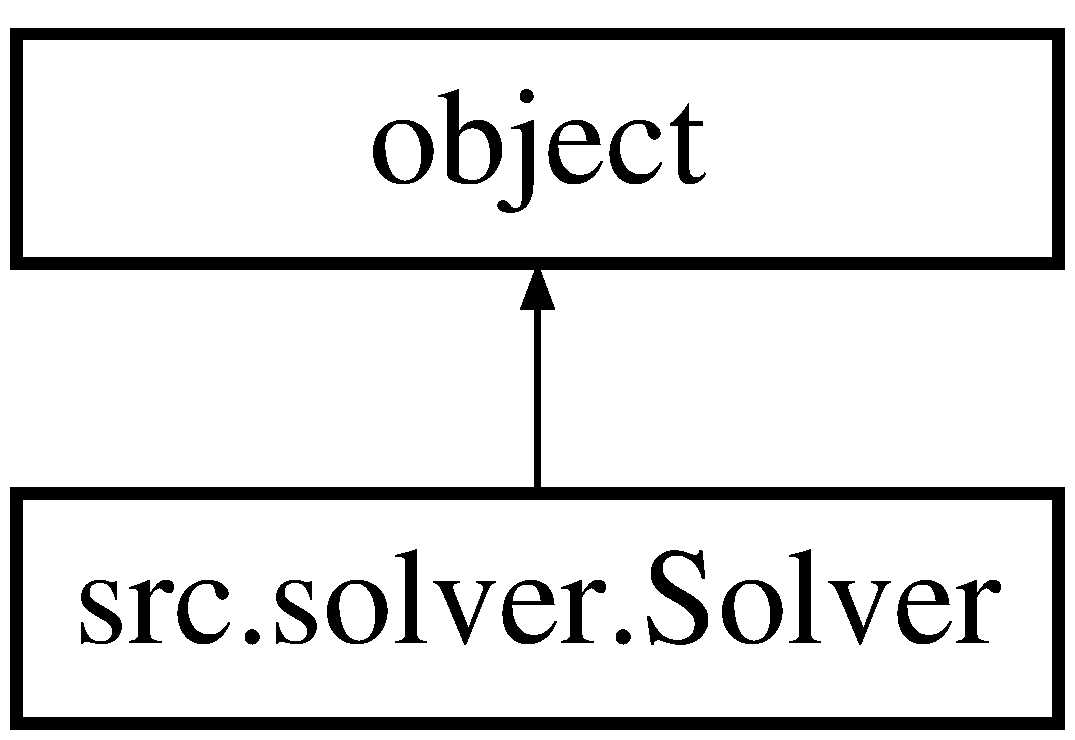
\includegraphics[height=2.000000cm]{classsrc_1_1solver_1_1Solver}
\end{center}
\end{figure}
\subsection*{Public Member Functions}
\begin{DoxyCompactItemize}
\item 
\mbox{\Hypertarget{classsrc_1_1solver_1_1Solver_aa4675ecd9497d24f63bc96467f8e07cd}\label{classsrc_1_1solver_1_1Solver_aa4675ecd9497d24f63bc96467f8e07cd}} 
def {\bfseries \+\_\+\+\_\+init\+\_\+\+\_\+} (self, model, data, kwargs)
\item 
\mbox{\Hypertarget{classsrc_1_1solver_1_1Solver_afde8803cac346c3ff7a4ac0adfa95e13}\label{classsrc_1_1solver_1_1Solver_afde8803cac346c3ff7a4ac0adfa95e13}} 
def {\bfseries train} (self)
\end{DoxyCompactItemize}
\subsection*{Public Attributes}
\begin{DoxyCompactItemize}
\item 
\mbox{\Hypertarget{classsrc_1_1solver_1_1Solver_a7386ec709398d24a7a80e59fd8fcb49d}\label{classsrc_1_1solver_1_1Solver_a7386ec709398d24a7a80e59fd8fcb49d}} 
{\bfseries model}
\item 
\mbox{\Hypertarget{classsrc_1_1solver_1_1Solver_a5bc6f71a6e206064d64be29318ea77d1}\label{classsrc_1_1solver_1_1Solver_a5bc6f71a6e206064d64be29318ea77d1}} 
{\bfseries X}
\item 
\mbox{\Hypertarget{classsrc_1_1solver_1_1Solver_a0e15601942ba7729575513e5240294cb}\label{classsrc_1_1solver_1_1Solver_a0e15601942ba7729575513e5240294cb}} 
{\bfseries update\+\_\+rule}
\item 
\mbox{\Hypertarget{classsrc_1_1solver_1_1Solver_a9a612f882172dcba38efc1b02d31d844}\label{classsrc_1_1solver_1_1Solver_a9a612f882172dcba38efc1b02d31d844}} 
{\bfseries optim\+\_\+config}
\item 
\mbox{\Hypertarget{classsrc_1_1solver_1_1Solver_a973b7f2e726bf033e5cbb0807a89ec71}\label{classsrc_1_1solver_1_1Solver_a973b7f2e726bf033e5cbb0807a89ec71}} 
{\bfseries batch\+\_\+size}
\item 
\mbox{\Hypertarget{classsrc_1_1solver_1_1Solver_af44b53f17c981c31e74799a6d64e4fac}\label{classsrc_1_1solver_1_1Solver_af44b53f17c981c31e74799a6d64e4fac}} 
{\bfseries num\+\_\+epochs}
\item 
\mbox{\Hypertarget{classsrc_1_1solver_1_1Solver_a0769cb1d0d167e0a3aba7d8a036716f3}\label{classsrc_1_1solver_1_1Solver_a0769cb1d0d167e0a3aba7d8a036716f3}} 
{\bfseries print\+\_\+every}
\item 
\mbox{\Hypertarget{classsrc_1_1solver_1_1Solver_a1f1e3c4c0485df56690c48684c2d0e01}\label{classsrc_1_1solver_1_1Solver_a1f1e3c4c0485df56690c48684c2d0e01}} 
{\bfseries epoch}
\item 
\mbox{\Hypertarget{classsrc_1_1solver_1_1Solver_a09eb5af6ea0d0f6c886bcd5772894bd7}\label{classsrc_1_1solver_1_1Solver_a09eb5af6ea0d0f6c886bcd5772894bd7}} 
{\bfseries loss\+\_\+history}
\item 
\mbox{\Hypertarget{classsrc_1_1solver_1_1Solver_a714be9061d3bef4402b7cdc77c237f0a}\label{classsrc_1_1solver_1_1Solver_a714be9061d3bef4402b7cdc77c237f0a}} 
{\bfseries optim\+\_\+configs}
\end{DoxyCompactItemize}


The documentation for this class was generated from the following file\+:\begin{DoxyCompactItemize}
\item 
/u/qingcanw/\+Programs/tsap/src/solver.\+py\end{DoxyCompactItemize}

\hypertarget{classtest_1_1testdataprocessor_1_1TestDataProcessor}{}\section{test.\+testdataprocessor.\+Test\+Data\+Processor Class Reference}
\label{classtest_1_1testdataprocessor_1_1TestDataProcessor}\index{test.\+testdataprocessor.\+Test\+Data\+Processor@{test.\+testdataprocessor.\+Test\+Data\+Processor}}
Inheritance diagram for test.\+testdataprocessor.\+Test\+Data\+Processor\+:\begin{figure}[H]
\begin{center}
\leavevmode
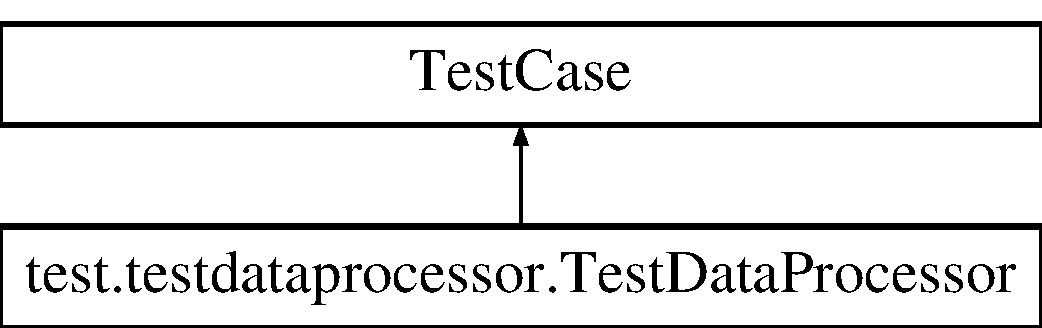
\includegraphics[height=2.000000cm]{classtest_1_1testdataprocessor_1_1TestDataProcessor}
\end{center}
\end{figure}
\subsection*{Public Member Functions}
\begin{DoxyCompactItemize}
\item 
def \hyperlink{classtest_1_1testdataprocessor_1_1TestDataProcessor_a6d0060026bc4963bf58c0fc502c1f647}{test\+Get\+Return1} (self)
\item 
def \hyperlink{classtest_1_1testdataprocessor_1_1TestDataProcessor_aa0451dcab76c90b2824fbc91c3f4bee0}{test\+Get\+Return2} (self)
\item 
def \hyperlink{classtest_1_1testdataprocessor_1_1TestDataProcessor_a6e171daffdd0608e5334d54795c20626}{test\+Get\+Return3} (self)
\item 
def \hyperlink{classtest_1_1testdataprocessor_1_1TestDataProcessor_af36dc7d2d905933ac59691b4609b74ce}{test\+Get\+Return4} (self)
\item 
def \hyperlink{classtest_1_1testdataprocessor_1_1TestDataProcessor_a5e277ac5b340c6bb491eff36a6000f56}{test\+Get\+Price1} (self)
\item 
def \hyperlink{classtest_1_1testdataprocessor_1_1TestDataProcessor_a2d042b3c50d860ddf2806be50318b6e3}{test\+Get\+Price2} (self)
\item 
def \hyperlink{classtest_1_1testdataprocessor_1_1TestDataProcessor_abea988851e0da77192e4048897006725}{test\+Get\+Price3} (self)
\item 
def \hyperlink{classtest_1_1testdataprocessor_1_1TestDataProcessor_a5b7943d1183bcd306163d4e50a469854}{test\+Max\+Drawdown1} (self)
\item 
def \hyperlink{classtest_1_1testdataprocessor_1_1TestDataProcessor_aca7fcd5ebc68735c66bdaf7ac498287a}{test\+Max\+Drawdown2} (self)
\item 
def \hyperlink{classtest_1_1testdataprocessor_1_1TestDataProcessor_a53255217d9105331fbd84eb51a7584e3}{test\+Max\+Drawdown3} (self)
\item 
def \hyperlink{classtest_1_1testdataprocessor_1_1TestDataProcessor_a8eb1635599669ec61f398acdef228665}{test\+Get\+Indicator1} (self)
\item 
def \hyperlink{classtest_1_1testdataprocessor_1_1TestDataProcessor_af49bbac371e28db7d98504e7ede06cca}{test\+Get\+Indicator2} (self)
\item 
def \hyperlink{classtest_1_1testdataprocessor_1_1TestDataProcessor_a8242e4dd97143e992bf624038265de2f}{test\+Get\+Indicator3} (self)
\item 
def \hyperlink{classtest_1_1testdataprocessor_1_1TestDataProcessor_a47dce81eea21d9be9b356d3a01009a00}{test\+Get\+Indicator4} (self)
\end{DoxyCompactItemize}


\subsection{Member Function Documentation}
\mbox{\Hypertarget{classtest_1_1testdataprocessor_1_1TestDataProcessor_a8eb1635599669ec61f398acdef228665}\label{classtest_1_1testdataprocessor_1_1TestDataProcessor_a8eb1635599669ec61f398acdef228665}} 
\index{test\+::testdataprocessor\+::\+Test\+Data\+Processor@{test\+::testdataprocessor\+::\+Test\+Data\+Processor}!test\+Get\+Indicator1@{test\+Get\+Indicator1}}
\index{test\+Get\+Indicator1@{test\+Get\+Indicator1}!test\+::testdataprocessor\+::\+Test\+Data\+Processor@{test\+::testdataprocessor\+::\+Test\+Data\+Processor}}
\subsubsection{\texorpdfstring{test\+Get\+Indicator1()}{testGetIndicator1()}}
{\footnotesize\ttfamily def test.\+testdataprocessor.\+Test\+Data\+Processor.\+test\+Get\+Indicator1 (\begin{DoxyParamCaption}\item[{}]{self }\end{DoxyParamCaption})}

\begin{DoxyVerb}test get_indicator with upper trend\end{DoxyVerb}
 \mbox{\Hypertarget{classtest_1_1testdataprocessor_1_1TestDataProcessor_af49bbac371e28db7d98504e7ede06cca}\label{classtest_1_1testdataprocessor_1_1TestDataProcessor_af49bbac371e28db7d98504e7ede06cca}} 
\index{test\+::testdataprocessor\+::\+Test\+Data\+Processor@{test\+::testdataprocessor\+::\+Test\+Data\+Processor}!test\+Get\+Indicator2@{test\+Get\+Indicator2}}
\index{test\+Get\+Indicator2@{test\+Get\+Indicator2}!test\+::testdataprocessor\+::\+Test\+Data\+Processor@{test\+::testdataprocessor\+::\+Test\+Data\+Processor}}
\subsubsection{\texorpdfstring{test\+Get\+Indicator2()}{testGetIndicator2()}}
{\footnotesize\ttfamily def test.\+testdataprocessor.\+Test\+Data\+Processor.\+test\+Get\+Indicator2 (\begin{DoxyParamCaption}\item[{}]{self }\end{DoxyParamCaption})}

\begin{DoxyVerb}test get_indicator with lower trend\end{DoxyVerb}
 \mbox{\Hypertarget{classtest_1_1testdataprocessor_1_1TestDataProcessor_a8242e4dd97143e992bf624038265de2f}\label{classtest_1_1testdataprocessor_1_1TestDataProcessor_a8242e4dd97143e992bf624038265de2f}} 
\index{test\+::testdataprocessor\+::\+Test\+Data\+Processor@{test\+::testdataprocessor\+::\+Test\+Data\+Processor}!test\+Get\+Indicator3@{test\+Get\+Indicator3}}
\index{test\+Get\+Indicator3@{test\+Get\+Indicator3}!test\+::testdataprocessor\+::\+Test\+Data\+Processor@{test\+::testdataprocessor\+::\+Test\+Data\+Processor}}
\subsubsection{\texorpdfstring{test\+Get\+Indicator3()}{testGetIndicator3()}}
{\footnotesize\ttfamily def test.\+testdataprocessor.\+Test\+Data\+Processor.\+test\+Get\+Indicator3 (\begin{DoxyParamCaption}\item[{}]{self }\end{DoxyParamCaption})}

\begin{DoxyVerb}test get_indicator without trend, trough before peak\end{DoxyVerb}
 \mbox{\Hypertarget{classtest_1_1testdataprocessor_1_1TestDataProcessor_a47dce81eea21d9be9b356d3a01009a00}\label{classtest_1_1testdataprocessor_1_1TestDataProcessor_a47dce81eea21d9be9b356d3a01009a00}} 
\index{test\+::testdataprocessor\+::\+Test\+Data\+Processor@{test\+::testdataprocessor\+::\+Test\+Data\+Processor}!test\+Get\+Indicator4@{test\+Get\+Indicator4}}
\index{test\+Get\+Indicator4@{test\+Get\+Indicator4}!test\+::testdataprocessor\+::\+Test\+Data\+Processor@{test\+::testdataprocessor\+::\+Test\+Data\+Processor}}
\subsubsection{\texorpdfstring{test\+Get\+Indicator4()}{testGetIndicator4()}}
{\footnotesize\ttfamily def test.\+testdataprocessor.\+Test\+Data\+Processor.\+test\+Get\+Indicator4 (\begin{DoxyParamCaption}\item[{}]{self }\end{DoxyParamCaption})}

\begin{DoxyVerb}test get_indicator without trend, trough after peak\end{DoxyVerb}
 \mbox{\Hypertarget{classtest_1_1testdataprocessor_1_1TestDataProcessor_a5e277ac5b340c6bb491eff36a6000f56}\label{classtest_1_1testdataprocessor_1_1TestDataProcessor_a5e277ac5b340c6bb491eff36a6000f56}} 
\index{test\+::testdataprocessor\+::\+Test\+Data\+Processor@{test\+::testdataprocessor\+::\+Test\+Data\+Processor}!test\+Get\+Price1@{test\+Get\+Price1}}
\index{test\+Get\+Price1@{test\+Get\+Price1}!test\+::testdataprocessor\+::\+Test\+Data\+Processor@{test\+::testdataprocessor\+::\+Test\+Data\+Processor}}
\subsubsection{\texorpdfstring{test\+Get\+Price1()}{testGetPrice1()}}
{\footnotesize\ttfamily def test.\+testdataprocessor.\+Test\+Data\+Processor.\+test\+Get\+Price1 (\begin{DoxyParamCaption}\item[{}]{self }\end{DoxyParamCaption})}

\begin{DoxyVerb}test get_price with a row vector whose elements are all 1.0\end{DoxyVerb}
 \mbox{\Hypertarget{classtest_1_1testdataprocessor_1_1TestDataProcessor_a2d042b3c50d860ddf2806be50318b6e3}\label{classtest_1_1testdataprocessor_1_1TestDataProcessor_a2d042b3c50d860ddf2806be50318b6e3}} 
\index{test\+::testdataprocessor\+::\+Test\+Data\+Processor@{test\+::testdataprocessor\+::\+Test\+Data\+Processor}!test\+Get\+Price2@{test\+Get\+Price2}}
\index{test\+Get\+Price2@{test\+Get\+Price2}!test\+::testdataprocessor\+::\+Test\+Data\+Processor@{test\+::testdataprocessor\+::\+Test\+Data\+Processor}}
\subsubsection{\texorpdfstring{test\+Get\+Price2()}{testGetPrice2()}}
{\footnotesize\ttfamily def test.\+testdataprocessor.\+Test\+Data\+Processor.\+test\+Get\+Price2 (\begin{DoxyParamCaption}\item[{}]{self }\end{DoxyParamCaption})}

\begin{DoxyVerb}test get_price with a row vector whose elements are not the same\end{DoxyVerb}
 \mbox{\Hypertarget{classtest_1_1testdataprocessor_1_1TestDataProcessor_abea988851e0da77192e4048897006725}\label{classtest_1_1testdataprocessor_1_1TestDataProcessor_abea988851e0da77192e4048897006725}} 
\index{test\+::testdataprocessor\+::\+Test\+Data\+Processor@{test\+::testdataprocessor\+::\+Test\+Data\+Processor}!test\+Get\+Price3@{test\+Get\+Price3}}
\index{test\+Get\+Price3@{test\+Get\+Price3}!test\+::testdataprocessor\+::\+Test\+Data\+Processor@{test\+::testdataprocessor\+::\+Test\+Data\+Processor}}
\subsubsection{\texorpdfstring{test\+Get\+Price3()}{testGetPrice3()}}
{\footnotesize\ttfamily def test.\+testdataprocessor.\+Test\+Data\+Processor.\+test\+Get\+Price3 (\begin{DoxyParamCaption}\item[{}]{self }\end{DoxyParamCaption})}

\begin{DoxyVerb}test get_price with a row vector whose elements are not the same, can be negative\end{DoxyVerb}
 \mbox{\Hypertarget{classtest_1_1testdataprocessor_1_1TestDataProcessor_a6d0060026bc4963bf58c0fc502c1f647}\label{classtest_1_1testdataprocessor_1_1TestDataProcessor_a6d0060026bc4963bf58c0fc502c1f647}} 
\index{test\+::testdataprocessor\+::\+Test\+Data\+Processor@{test\+::testdataprocessor\+::\+Test\+Data\+Processor}!test\+Get\+Return1@{test\+Get\+Return1}}
\index{test\+Get\+Return1@{test\+Get\+Return1}!test\+::testdataprocessor\+::\+Test\+Data\+Processor@{test\+::testdataprocessor\+::\+Test\+Data\+Processor}}
\subsubsection{\texorpdfstring{test\+Get\+Return1()}{testGetReturn1()}}
{\footnotesize\ttfamily def test.\+testdataprocessor.\+Test\+Data\+Processor.\+test\+Get\+Return1 (\begin{DoxyParamCaption}\item[{}]{self }\end{DoxyParamCaption})}

\begin{DoxyVerb}test get_return with a row vector whose elements are all 1.0\end{DoxyVerb}
 \mbox{\Hypertarget{classtest_1_1testdataprocessor_1_1TestDataProcessor_aa0451dcab76c90b2824fbc91c3f4bee0}\label{classtest_1_1testdataprocessor_1_1TestDataProcessor_aa0451dcab76c90b2824fbc91c3f4bee0}} 
\index{test\+::testdataprocessor\+::\+Test\+Data\+Processor@{test\+::testdataprocessor\+::\+Test\+Data\+Processor}!test\+Get\+Return2@{test\+Get\+Return2}}
\index{test\+Get\+Return2@{test\+Get\+Return2}!test\+::testdataprocessor\+::\+Test\+Data\+Processor@{test\+::testdataprocessor\+::\+Test\+Data\+Processor}}
\subsubsection{\texorpdfstring{test\+Get\+Return2()}{testGetReturn2()}}
{\footnotesize\ttfamily def test.\+testdataprocessor.\+Test\+Data\+Processor.\+test\+Get\+Return2 (\begin{DoxyParamCaption}\item[{}]{self }\end{DoxyParamCaption})}

\begin{DoxyVerb}test get_return with a row vector whose elements are not the same\end{DoxyVerb}
 \mbox{\Hypertarget{classtest_1_1testdataprocessor_1_1TestDataProcessor_a6e171daffdd0608e5334d54795c20626}\label{classtest_1_1testdataprocessor_1_1TestDataProcessor_a6e171daffdd0608e5334d54795c20626}} 
\index{test\+::testdataprocessor\+::\+Test\+Data\+Processor@{test\+::testdataprocessor\+::\+Test\+Data\+Processor}!test\+Get\+Return3@{test\+Get\+Return3}}
\index{test\+Get\+Return3@{test\+Get\+Return3}!test\+::testdataprocessor\+::\+Test\+Data\+Processor@{test\+::testdataprocessor\+::\+Test\+Data\+Processor}}
\subsubsection{\texorpdfstring{test\+Get\+Return3()}{testGetReturn3()}}
{\footnotesize\ttfamily def test.\+testdataprocessor.\+Test\+Data\+Processor.\+test\+Get\+Return3 (\begin{DoxyParamCaption}\item[{}]{self }\end{DoxyParamCaption})}

\begin{DoxyVerb}test get_return with a matrix\end{DoxyVerb}
 \mbox{\Hypertarget{classtest_1_1testdataprocessor_1_1TestDataProcessor_af36dc7d2d905933ac59691b4609b74ce}\label{classtest_1_1testdataprocessor_1_1TestDataProcessor_af36dc7d2d905933ac59691b4609b74ce}} 
\index{test\+::testdataprocessor\+::\+Test\+Data\+Processor@{test\+::testdataprocessor\+::\+Test\+Data\+Processor}!test\+Get\+Return4@{test\+Get\+Return4}}
\index{test\+Get\+Return4@{test\+Get\+Return4}!test\+::testdataprocessor\+::\+Test\+Data\+Processor@{test\+::testdataprocessor\+::\+Test\+Data\+Processor}}
\subsubsection{\texorpdfstring{test\+Get\+Return4()}{testGetReturn4()}}
{\footnotesize\ttfamily def test.\+testdataprocessor.\+Test\+Data\+Processor.\+test\+Get\+Return4 (\begin{DoxyParamCaption}\item[{}]{self }\end{DoxyParamCaption})}

\begin{DoxyVerb}test get_return with a larger matrix\end{DoxyVerb}
 \mbox{\Hypertarget{classtest_1_1testdataprocessor_1_1TestDataProcessor_a5b7943d1183bcd306163d4e50a469854}\label{classtest_1_1testdataprocessor_1_1TestDataProcessor_a5b7943d1183bcd306163d4e50a469854}} 
\index{test\+::testdataprocessor\+::\+Test\+Data\+Processor@{test\+::testdataprocessor\+::\+Test\+Data\+Processor}!test\+Max\+Drawdown1@{test\+Max\+Drawdown1}}
\index{test\+Max\+Drawdown1@{test\+Max\+Drawdown1}!test\+::testdataprocessor\+::\+Test\+Data\+Processor@{test\+::testdataprocessor\+::\+Test\+Data\+Processor}}
\subsubsection{\texorpdfstring{test\+Max\+Drawdown1()}{testMaxDrawdown1()}}
{\footnotesize\ttfamily def test.\+testdataprocessor.\+Test\+Data\+Processor.\+test\+Max\+Drawdown1 (\begin{DoxyParamCaption}\item[{}]{self }\end{DoxyParamCaption})}

\begin{DoxyVerb}test max_drawdown with upper trend\end{DoxyVerb}
 \mbox{\Hypertarget{classtest_1_1testdataprocessor_1_1TestDataProcessor_aca7fcd5ebc68735c66bdaf7ac498287a}\label{classtest_1_1testdataprocessor_1_1TestDataProcessor_aca7fcd5ebc68735c66bdaf7ac498287a}} 
\index{test\+::testdataprocessor\+::\+Test\+Data\+Processor@{test\+::testdataprocessor\+::\+Test\+Data\+Processor}!test\+Max\+Drawdown2@{test\+Max\+Drawdown2}}
\index{test\+Max\+Drawdown2@{test\+Max\+Drawdown2}!test\+::testdataprocessor\+::\+Test\+Data\+Processor@{test\+::testdataprocessor\+::\+Test\+Data\+Processor}}
\subsubsection{\texorpdfstring{test\+Max\+Drawdown2()}{testMaxDrawdown2()}}
{\footnotesize\ttfamily def test.\+testdataprocessor.\+Test\+Data\+Processor.\+test\+Max\+Drawdown2 (\begin{DoxyParamCaption}\item[{}]{self }\end{DoxyParamCaption})}

\begin{DoxyVerb}test max_drawdown with lower trend\end{DoxyVerb}
 \mbox{\Hypertarget{classtest_1_1testdataprocessor_1_1TestDataProcessor_a53255217d9105331fbd84eb51a7584e3}\label{classtest_1_1testdataprocessor_1_1TestDataProcessor_a53255217d9105331fbd84eb51a7584e3}} 
\index{test\+::testdataprocessor\+::\+Test\+Data\+Processor@{test\+::testdataprocessor\+::\+Test\+Data\+Processor}!test\+Max\+Drawdown3@{test\+Max\+Drawdown3}}
\index{test\+Max\+Drawdown3@{test\+Max\+Drawdown3}!test\+::testdataprocessor\+::\+Test\+Data\+Processor@{test\+::testdataprocessor\+::\+Test\+Data\+Processor}}
\subsubsection{\texorpdfstring{test\+Max\+Drawdown3()}{testMaxDrawdown3()}}
{\footnotesize\ttfamily def test.\+testdataprocessor.\+Test\+Data\+Processor.\+test\+Max\+Drawdown3 (\begin{DoxyParamCaption}\item[{}]{self }\end{DoxyParamCaption})}

\begin{DoxyVerb}test max_drawdown with peak and trough\end{DoxyVerb}
 

The documentation for this class was generated from the following file\+:\begin{DoxyCompactItemize}
\item 
/u/qingcanw/\+Programs/tsap/test/testdataprocessor.\+py\end{DoxyCompactItemize}

\hypertarget{classtest_1_1testmodel_1_1TestModel}{}\section{test.\+testmodel.\+Test\+Model Class Reference}
\label{classtest_1_1testmodel_1_1TestModel}\index{test.\+testmodel.\+Test\+Model@{test.\+testmodel.\+Test\+Model}}
Inheritance diagram for test.\+testmodel.\+Test\+Model\+:\begin{figure}[H]
\begin{center}
\leavevmode
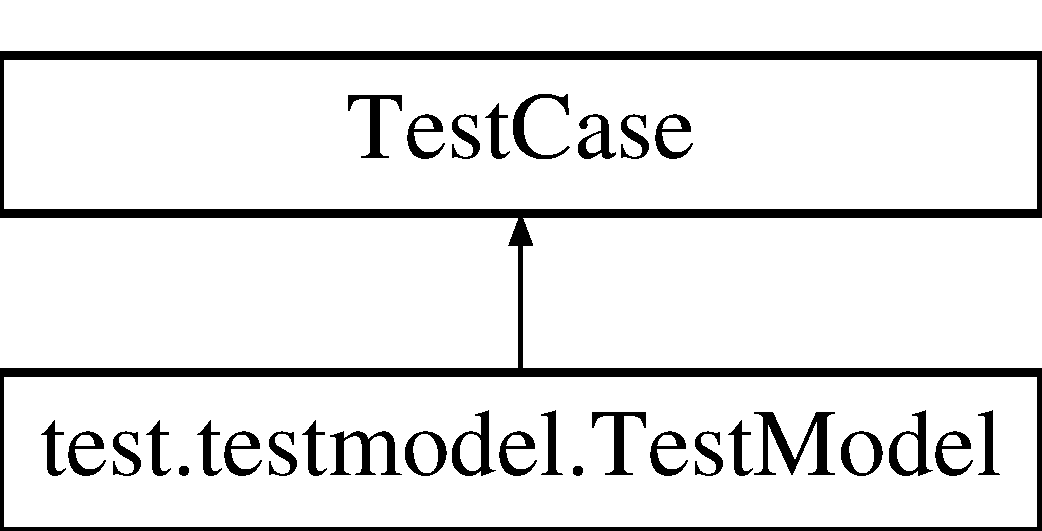
\includegraphics[height=2.000000cm]{classtest_1_1testmodel_1_1TestModel}
\end{center}
\end{figure}
\subsection*{Public Member Functions}
\begin{DoxyCompactItemize}
\item 
\mbox{\Hypertarget{classtest_1_1testmodel_1_1TestModel_a547a64497746faf47c4a522431033233}\label{classtest_1_1testmodel_1_1TestModel_a547a64497746faf47c4a522431033233}} 
def {\bfseries test\+A\+Rloglklh1} (self)
\item 
\mbox{\Hypertarget{classtest_1_1testmodel_1_1TestModel_a3560e3dc4662df6986dc8b48dd81a421}\label{classtest_1_1testmodel_1_1TestModel_a3560e3dc4662df6986dc8b48dd81a421}} 
def {\bfseries test\+A\+Rlklh2} (self)
\item 
\mbox{\Hypertarget{classtest_1_1testmodel_1_1TestModel_a8f40fb31c306f9969520fc9bf8a7ffd1}\label{classtest_1_1testmodel_1_1TestModel_a8f40fb31c306f9969520fc9bf8a7ffd1}} 
def {\bfseries test\+A\+Rgrad1} (self)
\item 
\mbox{\Hypertarget{classtest_1_1testmodel_1_1TestModel_a3f3cfe951bf743e47169ca992e25b285}\label{classtest_1_1testmodel_1_1TestModel_a3f3cfe951bf743e47169ca992e25b285}} 
def {\bfseries test\+A\+Rgrad2} (self)
\item 
\mbox{\Hypertarget{classtest_1_1testmodel_1_1TestModel_ad4a36eaadbdd8e1d0f4600f24a0c850d}\label{classtest_1_1testmodel_1_1TestModel_ad4a36eaadbdd8e1d0f4600f24a0c850d}} 
def {\bfseries test\+M\+Aloglklh1} (self)
\item 
\mbox{\Hypertarget{classtest_1_1testmodel_1_1TestModel_a117218d6206e5ca859e9b376739552f7}\label{classtest_1_1testmodel_1_1TestModel_a117218d6206e5ca859e9b376739552f7}} 
def {\bfseries test\+M\+Aloglklh2} (self)
\end{DoxyCompactItemize}


The documentation for this class was generated from the following file\+:\begin{DoxyCompactItemize}
\item 
/u/qingcanw/\+Programs/tsap/test/testmodel.\+py\end{DoxyCompactItemize}

\hypertarget{classtest_1_1testtrading_1_1TestTrading}{}\section{test.\+testtrading.\+Test\+Trading Class Reference}
\label{classtest_1_1testtrading_1_1TestTrading}\index{test.\+testtrading.\+Test\+Trading@{test.\+testtrading.\+Test\+Trading}}
Inheritance diagram for test.\+testtrading.\+Test\+Trading\+:\begin{figure}[H]
\begin{center}
\leavevmode
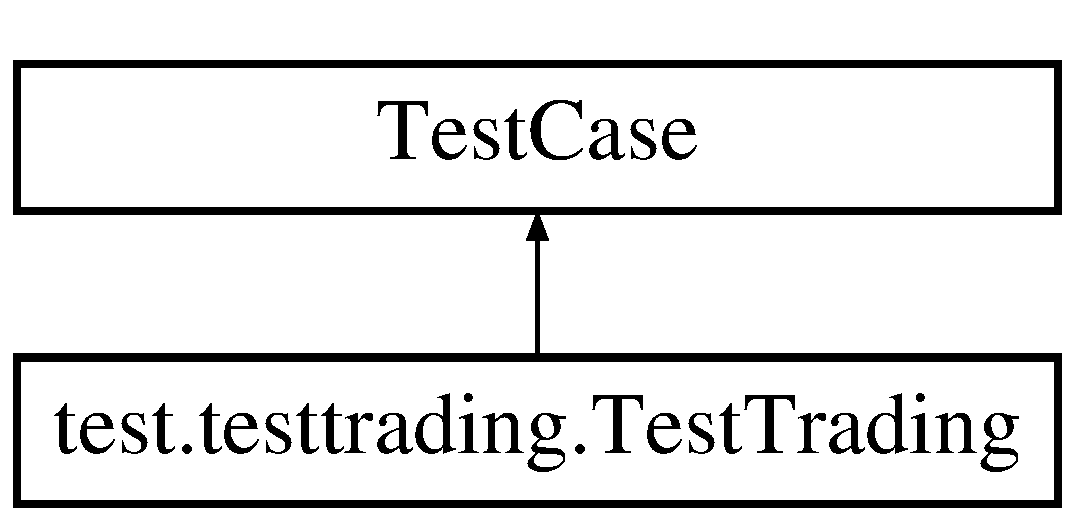
\includegraphics[height=2.000000cm]{classtest_1_1testtrading_1_1TestTrading}
\end{center}
\end{figure}
\subsection*{Public Member Functions}
\begin{DoxyCompactItemize}
\item 
def \hyperlink{classtest_1_1testtrading_1_1TestTrading_a428be4083e5f6130022d680385742c37}{test\+Signal\+Generation1} (self)
\item 
def \hyperlink{classtest_1_1testtrading_1_1TestTrading_a0a3a1e94ab4195b6eb4cf6f8a3e96a11}{test\+Signal\+Generation2} (self)
\item 
def \hyperlink{classtest_1_1testtrading_1_1TestTrading_af42ccddb031cfaa9662efa049fba073d}{test\+Signal\+Generation3} (self)
\item 
def \hyperlink{classtest_1_1testtrading_1_1TestTrading_a3bb0a3ee69ffdb02c45c76cec97dfe46}{test\+Signal\+Generation4} (self)
\item 
def \hyperlink{classtest_1_1testtrading_1_1TestTrading_a1314bb991d7ae8a7f0bb708392be6b8f}{test\+Signal\+Generation5} (self)
\item 
def \hyperlink{classtest_1_1testtrading_1_1TestTrading_ae24881ed7effd9e9cd012a8bce93ff18}{test\+Profit\+Loss1} (self)
\item 
def \hyperlink{classtest_1_1testtrading_1_1TestTrading_aed815691829a73306aa7f17bd6b95c3b}{test\+Profit\+Loss2} (self)
\item 
def \hyperlink{classtest_1_1testtrading_1_1TestTrading_a996cc7999e191d67410789030eabdf1c}{test\+Profit\+Loss3} (self)
\item 
def \hyperlink{classtest_1_1testtrading_1_1TestTrading_af3110d4d491f6d1a4cc67916c6c189a2}{test\+Profit\+Loss4} (self)
\item 
def \hyperlink{classtest_1_1testtrading_1_1TestTrading_a4684dd9999fdf9a9c7e898f6a617c1f3}{test\+Trade1} (self)
\end{DoxyCompactItemize}


\subsection{Member Function Documentation}
\mbox{\Hypertarget{classtest_1_1testtrading_1_1TestTrading_ae24881ed7effd9e9cd012a8bce93ff18}\label{classtest_1_1testtrading_1_1TestTrading_ae24881ed7effd9e9cd012a8bce93ff18}} 
\index{test\+::testtrading\+::\+Test\+Trading@{test\+::testtrading\+::\+Test\+Trading}!test\+Profit\+Loss1@{test\+Profit\+Loss1}}
\index{test\+Profit\+Loss1@{test\+Profit\+Loss1}!test\+::testtrading\+::\+Test\+Trading@{test\+::testtrading\+::\+Test\+Trading}}
\subsubsection{\texorpdfstring{test\+Profit\+Loss1()}{testProfitLoss1()}}
{\footnotesize\ttfamily def test.\+testtrading.\+Test\+Trading.\+test\+Profit\+Loss1 (\begin{DoxyParamCaption}\item[{}]{self }\end{DoxyParamCaption})}

\begin{DoxyVerb}test profit_loss with upper trend, this is immediate buy\end{DoxyVerb}
 \mbox{\Hypertarget{classtest_1_1testtrading_1_1TestTrading_aed815691829a73306aa7f17bd6b95c3b}\label{classtest_1_1testtrading_1_1TestTrading_aed815691829a73306aa7f17bd6b95c3b}} 
\index{test\+::testtrading\+::\+Test\+Trading@{test\+::testtrading\+::\+Test\+Trading}!test\+Profit\+Loss2@{test\+Profit\+Loss2}}
\index{test\+Profit\+Loss2@{test\+Profit\+Loss2}!test\+::testtrading\+::\+Test\+Trading@{test\+::testtrading\+::\+Test\+Trading}}
\subsubsection{\texorpdfstring{test\+Profit\+Loss2()}{testProfitLoss2()}}
{\footnotesize\ttfamily def test.\+testtrading.\+Test\+Trading.\+test\+Profit\+Loss2 (\begin{DoxyParamCaption}\item[{}]{self }\end{DoxyParamCaption})}

\begin{DoxyVerb}test profit_loss with upper trend, this is immediate buy\end{DoxyVerb}
 \mbox{\Hypertarget{classtest_1_1testtrading_1_1TestTrading_a996cc7999e191d67410789030eabdf1c}\label{classtest_1_1testtrading_1_1TestTrading_a996cc7999e191d67410789030eabdf1c}} 
\index{test\+::testtrading\+::\+Test\+Trading@{test\+::testtrading\+::\+Test\+Trading}!test\+Profit\+Loss3@{test\+Profit\+Loss3}}
\index{test\+Profit\+Loss3@{test\+Profit\+Loss3}!test\+::testtrading\+::\+Test\+Trading@{test\+::testtrading\+::\+Test\+Trading}}
\subsubsection{\texorpdfstring{test\+Profit\+Loss3()}{testProfitLoss3()}}
{\footnotesize\ttfamily def test.\+testtrading.\+Test\+Trading.\+test\+Profit\+Loss3 (\begin{DoxyParamCaption}\item[{}]{self }\end{DoxyParamCaption})}

\begin{DoxyVerb}test profit_loss with longer holding period\end{DoxyVerb}
 \mbox{\Hypertarget{classtest_1_1testtrading_1_1TestTrading_af3110d4d491f6d1a4cc67916c6c189a2}\label{classtest_1_1testtrading_1_1TestTrading_af3110d4d491f6d1a4cc67916c6c189a2}} 
\index{test\+::testtrading\+::\+Test\+Trading@{test\+::testtrading\+::\+Test\+Trading}!test\+Profit\+Loss4@{test\+Profit\+Loss4}}
\index{test\+Profit\+Loss4@{test\+Profit\+Loss4}!test\+::testtrading\+::\+Test\+Trading@{test\+::testtrading\+::\+Test\+Trading}}
\subsubsection{\texorpdfstring{test\+Profit\+Loss4()}{testProfitLoss4()}}
{\footnotesize\ttfamily def test.\+testtrading.\+Test\+Trading.\+test\+Profit\+Loss4 (\begin{DoxyParamCaption}\item[{}]{self }\end{DoxyParamCaption})}

\begin{DoxyVerb}test profit_loss with longer holding period, multiple trades and more money\end{DoxyVerb}
 \mbox{\Hypertarget{classtest_1_1testtrading_1_1TestTrading_a428be4083e5f6130022d680385742c37}\label{classtest_1_1testtrading_1_1TestTrading_a428be4083e5f6130022d680385742c37}} 
\index{test\+::testtrading\+::\+Test\+Trading@{test\+::testtrading\+::\+Test\+Trading}!test\+Signal\+Generation1@{test\+Signal\+Generation1}}
\index{test\+Signal\+Generation1@{test\+Signal\+Generation1}!test\+::testtrading\+::\+Test\+Trading@{test\+::testtrading\+::\+Test\+Trading}}
\subsubsection{\texorpdfstring{test\+Signal\+Generation1()}{testSignalGeneration1()}}
{\footnotesize\ttfamily def test.\+testtrading.\+Test\+Trading.\+test\+Signal\+Generation1 (\begin{DoxyParamCaption}\item[{}]{self }\end{DoxyParamCaption})}

\begin{DoxyVerb}test signal_generation with upper trend\end{DoxyVerb}
 \mbox{\Hypertarget{classtest_1_1testtrading_1_1TestTrading_a0a3a1e94ab4195b6eb4cf6f8a3e96a11}\label{classtest_1_1testtrading_1_1TestTrading_a0a3a1e94ab4195b6eb4cf6f8a3e96a11}} 
\index{test\+::testtrading\+::\+Test\+Trading@{test\+::testtrading\+::\+Test\+Trading}!test\+Signal\+Generation2@{test\+Signal\+Generation2}}
\index{test\+Signal\+Generation2@{test\+Signal\+Generation2}!test\+::testtrading\+::\+Test\+Trading@{test\+::testtrading\+::\+Test\+Trading}}
\subsubsection{\texorpdfstring{test\+Signal\+Generation2()}{testSignalGeneration2()}}
{\footnotesize\ttfamily def test.\+testtrading.\+Test\+Trading.\+test\+Signal\+Generation2 (\begin{DoxyParamCaption}\item[{}]{self }\end{DoxyParamCaption})}

\begin{DoxyVerb}test signal_generation with lower trend\end{DoxyVerb}
 \mbox{\Hypertarget{classtest_1_1testtrading_1_1TestTrading_af42ccddb031cfaa9662efa049fba073d}\label{classtest_1_1testtrading_1_1TestTrading_af42ccddb031cfaa9662efa049fba073d}} 
\index{test\+::testtrading\+::\+Test\+Trading@{test\+::testtrading\+::\+Test\+Trading}!test\+Signal\+Generation3@{test\+Signal\+Generation3}}
\index{test\+Signal\+Generation3@{test\+Signal\+Generation3}!test\+::testtrading\+::\+Test\+Trading@{test\+::testtrading\+::\+Test\+Trading}}
\subsubsection{\texorpdfstring{test\+Signal\+Generation3()}{testSignalGeneration3()}}
{\footnotesize\ttfamily def test.\+testtrading.\+Test\+Trading.\+test\+Signal\+Generation3 (\begin{DoxyParamCaption}\item[{}]{self }\end{DoxyParamCaption})}

\begin{DoxyVerb}test signal_generation without trend\end{DoxyVerb}
 \mbox{\Hypertarget{classtest_1_1testtrading_1_1TestTrading_a3bb0a3ee69ffdb02c45c76cec97dfe46}\label{classtest_1_1testtrading_1_1TestTrading_a3bb0a3ee69ffdb02c45c76cec97dfe46}} 
\index{test\+::testtrading\+::\+Test\+Trading@{test\+::testtrading\+::\+Test\+Trading}!test\+Signal\+Generation4@{test\+Signal\+Generation4}}
\index{test\+Signal\+Generation4@{test\+Signal\+Generation4}!test\+::testtrading\+::\+Test\+Trading@{test\+::testtrading\+::\+Test\+Trading}}
\subsubsection{\texorpdfstring{test\+Signal\+Generation4()}{testSignalGeneration4()}}
{\footnotesize\ttfamily def test.\+testtrading.\+Test\+Trading.\+test\+Signal\+Generation4 (\begin{DoxyParamCaption}\item[{}]{self }\end{DoxyParamCaption})}

\begin{DoxyVerb}test signal_generation with bigger window\end{DoxyVerb}
 \mbox{\Hypertarget{classtest_1_1testtrading_1_1TestTrading_a1314bb991d7ae8a7f0bb708392be6b8f}\label{classtest_1_1testtrading_1_1TestTrading_a1314bb991d7ae8a7f0bb708392be6b8f}} 
\index{test\+::testtrading\+::\+Test\+Trading@{test\+::testtrading\+::\+Test\+Trading}!test\+Signal\+Generation5@{test\+Signal\+Generation5}}
\index{test\+Signal\+Generation5@{test\+Signal\+Generation5}!test\+::testtrading\+::\+Test\+Trading@{test\+::testtrading\+::\+Test\+Trading}}
\subsubsection{\texorpdfstring{test\+Signal\+Generation5()}{testSignalGeneration5()}}
{\footnotesize\ttfamily def test.\+testtrading.\+Test\+Trading.\+test\+Signal\+Generation5 (\begin{DoxyParamCaption}\item[{}]{self }\end{DoxyParamCaption})}

\begin{DoxyVerb}test signal_generation with bigger holding period\end{DoxyVerb}
 \mbox{\Hypertarget{classtest_1_1testtrading_1_1TestTrading_a4684dd9999fdf9a9c7e898f6a617c1f3}\label{classtest_1_1testtrading_1_1TestTrading_a4684dd9999fdf9a9c7e898f6a617c1f3}} 
\index{test\+::testtrading\+::\+Test\+Trading@{test\+::testtrading\+::\+Test\+Trading}!test\+Trade1@{test\+Trade1}}
\index{test\+Trade1@{test\+Trade1}!test\+::testtrading\+::\+Test\+Trading@{test\+::testtrading\+::\+Test\+Trading}}
\subsubsection{\texorpdfstring{test\+Trade1()}{testTrade1()}}
{\footnotesize\ttfamily def test.\+testtrading.\+Test\+Trading.\+test\+Trade1 (\begin{DoxyParamCaption}\item[{}]{self }\end{DoxyParamCaption})}

\begin{DoxyVerb}test trade with a very simple model\end{DoxyVerb}
 

The documentation for this class was generated from the following file\+:\begin{DoxyCompactItemize}
\item 
/u/qingcanw/\+Programs/tsap/test/testtrading.\+py\end{DoxyCompactItemize}

%--- End generated contents ---

% Index
\backmatter
\newpage
\phantomsection
\clearemptydoublepage
\addcontentsline{toc}{chapter}{Index}
\printindex

\end{document}
